% Options for packages loaded elsewhere
\PassOptionsToPackage{unicode}{hyperref}
\PassOptionsToPackage{hyphens}{url}
%
\documentclass[
  11pt,
]{article}
\title{Competition fails mass transit: The Case of a Megacity in the
Developing world}
\author{true}
\date{July 14, 2021}

\usepackage{amsmath,amssymb}
\usepackage[]{mathpazo}
\usepackage{iftex}
\ifPDFTeX
  \usepackage[T1]{fontenc}
  \usepackage[utf8]{inputenc}
  \usepackage{textcomp} % provide euro and other symbols
\else % if luatex or xetex
  \usepackage{unicode-math}
  \defaultfontfeatures{Scale=MatchLowercase}
  \defaultfontfeatures[\rmfamily]{Ligatures=TeX,Scale=1}
\fi
% Use upquote if available, for straight quotes in verbatim environments
\IfFileExists{upquote.sty}{\usepackage{upquote}}{}
\IfFileExists{microtype.sty}{% use microtype if available
  \usepackage[]{microtype}
  \UseMicrotypeSet[protrusion]{basicmath} % disable protrusion for tt fonts
}{}
\makeatletter
\@ifundefined{KOMAClassName}{% if non-KOMA class
  \IfFileExists{parskip.sty}{%
    \usepackage{parskip}
  }{% else
    \setlength{\parindent}{0pt}
    \setlength{\parskip}{6pt plus 2pt minus 1pt}}
}{% if KOMA class
  \KOMAoptions{parskip=half}}
\makeatother
\usepackage{xcolor}
\IfFileExists{xurl.sty}{\usepackage{xurl}}{} % add URL line breaks if available
\IfFileExists{bookmark.sty}{\usepackage{bookmark}}{\usepackage{hyperref}}
\hypersetup{
  pdftitle={Competition fails mass transit: The Case of a Megacity in the Developing world},
  pdfkeywords={mass transportation, South Asia, Political economy},
  hidelinks,
  pdfcreator={LaTeX via pandoc}}
\urlstyle{same} % disable monospaced font for URLs
\usepackage[margin=1in]{geometry}
\usepackage{graphicx}
\makeatletter
\def\maxwidth{\ifdim\Gin@nat@width>\linewidth\linewidth\else\Gin@nat@width\fi}
\def\maxheight{\ifdim\Gin@nat@height>\textheight\textheight\else\Gin@nat@height\fi}
\makeatother
% Scale images if necessary, so that they will not overflow the page
% margins by default, and it is still possible to overwrite the defaults
% using explicit options in \includegraphics[width, height, ...]{}
\setkeys{Gin}{width=\maxwidth,height=\maxheight,keepaspectratio}
% Set default figure placement to htbp
\makeatletter
\def\fps@figure{htbp}
\makeatother
\setlength{\emergencystretch}{3em} % prevent overfull lines
\providecommand{\tightlist}{%
  \setlength{\itemsep}{0pt}\setlength{\parskip}{0pt}}
\setcounter{secnumdepth}{-\maxdimen} % remove section numbering
\usepackage[format=hang,labelformat=empty,labelsep=none]{caption}
%\usepackage{fontspec}
\usepackage{newpxtext}
\usepackage{wrapfig}
%\usepackage{biblatex}
%\addbibresource{../../References/masterRefs.bib}
\usepackage{float}
\let\origfigure\figure
\let\endorigfigure\endfigure
\renewenvironment{figure}[1][2] {
    \expandafter\origfigure\expandafter[H]
} {
    \endorigfigure
}
%\usepackage{draftwatermark}
%\SetWatermarkLightness{.9}
\def\tightlist{}
\ifLuaTeX
  \usepackage{selnolig}  % disable illegal ligatures
\fi
\usepackage[style=authoryear,]{biblatex}
\addbibresource{../References/masterRefs.bib}

\begin{document}
\maketitle
\begin{abstract}
This article will analyze the dynamics and structure of mass
transportation in a South Asian mega city.It is usually expected that
competition will bring about better service and quality in a market. In
transportation sector in Bangladesh it seemed that competion brought
about the worst possible outcome for transportation. This paper
investigates the reasons behind this phenomenon. We found that this is
actually a classic case of market failure since mass transportation is
essentially a public good with externality effect. Therefore, market
equilibrium resulted into socially inefficient outcome.
\end{abstract}

\hypertarget{introduction}{%
\section{Introduction}\label{introduction}}

It was a sultry summer afternoon on 29th July of 2018. Two students of
capital city of Bangladesh, Dhaka was waiting on the roadside of a busy
major road. Then according to eye witness, a speeding car lost control
and ran over those two hapless students. They were dead on the spot.

This tragic event instigated a unique movement in the streets of Dhaka,
Bangladesh. It brought about protests throughout the country and
particularly in Dhaka, the school students took over the control of the
streets replacing the traffic police. It created a great political
upheaval in Bangladesh. High school kids, secondary school kids came to
streets protesting death of two of their friends. This kids actually
ruled the city for a few days, controlling traffics. This protests
finally ended after a week or so amidst government crackdown which
allegedly through human rights abuse. But it captured a big part of
public imagination and is believed to remain in public memory for a long
time.

It was a common incident that Bus drivers are quite reckless. That was
not the first time it happened. Frequently these city buses were
involved in several accidents. People were already pissed off.
Therefore, when kids got involved it became very sensitive.

With this background, we would like to investigate whether mass
transportation, particularly Bus service is problematic or not. It is
apparent this sector is quite competitive. There are quite a few actors
in the market. Bus drivers compete with each other to pick up passengers
and finish the trip earlier.

It is usually expected that competition will bring about better service
and quality in a market. In transportation sector in Bangladesh it
seemed that competition brought about the worst possible outcome for
transportation. This paper investigates the reasons behind this
phenomenon. We found that this is actually a classic case of market
failure since mass transportation is essentially a public good with
externality effect. Therefore, market equilibrium resulted into socially
inefficient outcome. A related objective of this paper is to look into
the economic incentive of Bus operators that lead to this stiff
aggressively competitive behaviors which led to the tragic incident. We
will look into the current employment structure which is actually
determined by the whole mass transportation industry.

\hypertarget{transporation-infrastructre}{%
\section{Transporation
infrastructre}\label{transporation-infrastructre}}

First start with an small intro of dhaka. then talk about the population
size, how fast it is growing. then talk about modal share and show the
importance of bus.

Dhaka is one of the megacities in the world. Currently its rank is this.
It has population of 14.8 million. The area of Dhaka can be defined in
various ways.

\begin{wrapfigure}{l}{.35\textwidth}  
 \begin{center}
    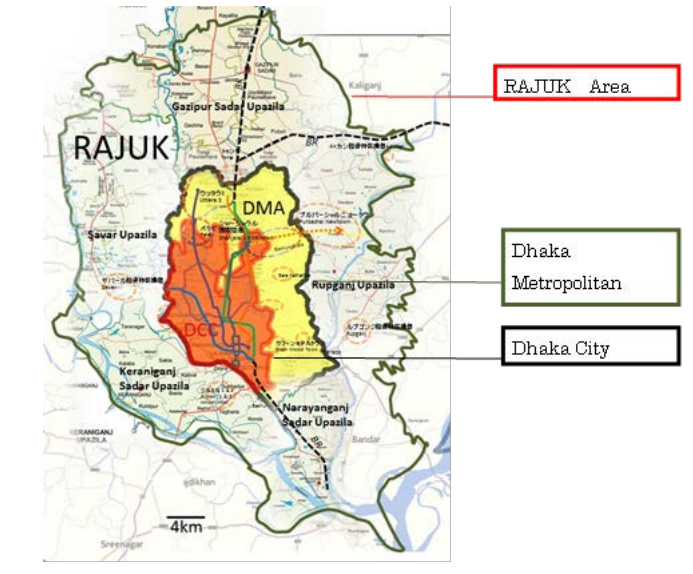
\includegraphics{./figures/dma.png}  
  \caption{Dhaka metropolitan area} 
\end{center}
\end{wrapfigure}

The population in the above area growing very fast. To meet the daily
needs of this high population, at present, there are about 30 million
trips produced per day in Dhaka. The transportation of this huge
population is dependent on bus. Let's have a look at the following
figures.

The population in the above area growing very fast. To meet the daily
needs of this high population, at present, there are about 30 million
trips produced per day in Dhaka. The transportation of this huge
population is dependent on bus. Let's have a look at the following
figures.

\begin{wrapfigure}{r}{.4\textwidth}  
 \begin{center}
    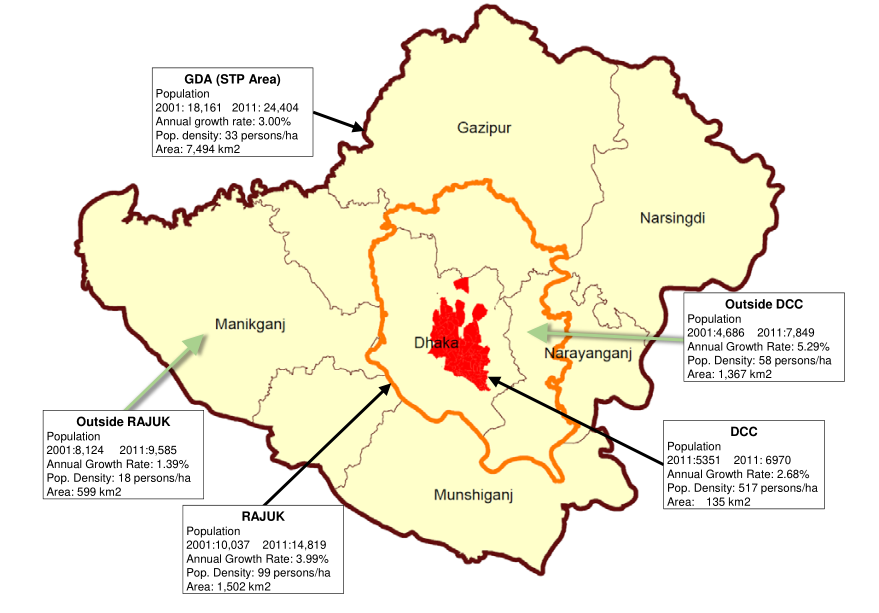
\includegraphics{./figures/gda.png}  
  \caption{Greater Dhaka area} 
\end{center}
\end{wrapfigure}

Mini-bus is a shorter version bus which can not carry more than 30
passengers. If it can carry more than 30 passengers then it is a bus.

there are 3.30 million vehicles in the country. There are total 35,000
buses and mini buses and half of these vehicles are concentrated in
Dhaka. In Dhaka there are around 9000 bus and mini buses operate.

The above figures shows that bus is the dominant form of transportation
in Dhaka city (\textbf{Describe more on modal share}). According to BRTA
\textbf{fix the reference} there are 3.30 million vehicles in the
country. There are total 35,000 buses and mini buses and half of these
vehicles are concentrated in Dhaka. In Dhaka there are around 9000 bus
and mini buses operate.

These buses operate very strangely in Dhaka. The determination of bus
routes is very haphazard. In owes back to the way the routes has been
evoloved in Dhaka. For example, in 1992, in Dhaka city there were only
27 bus routes. During that period, there were 304 buses were in
operation (DITS, 1994).

\begin{wrapfigure}{l}{.4\textwidth}  
 \begin{center}
    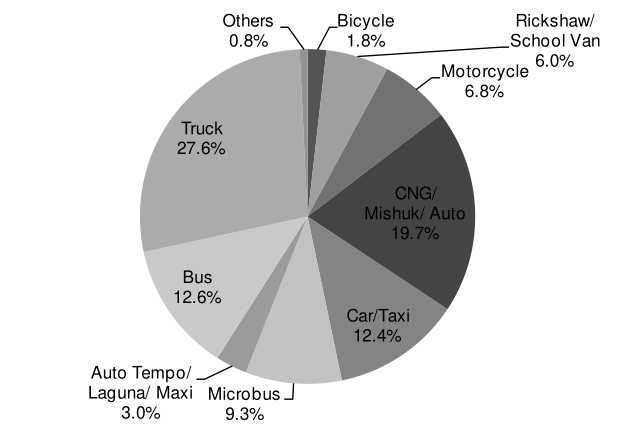
\includegraphics{./figures/rstp_modal_share_traffic.png}  
  \caption{Modal share} 
\end{center}
\end{wrapfigure}

These buses has to take permission from Dhaka Metropolitan Regional
transport committee for designated routes. Motor vehicle act play a key
role in the application for route process. But unfortunately the other
key factors such as passenger demand, the density of route with other
buses are not considered. It is also learnt that political and clouts of
the applicant also pay a great role here.

\begin{wrapfigure}{r}{.4\textwidth}  
 \begin{center}
    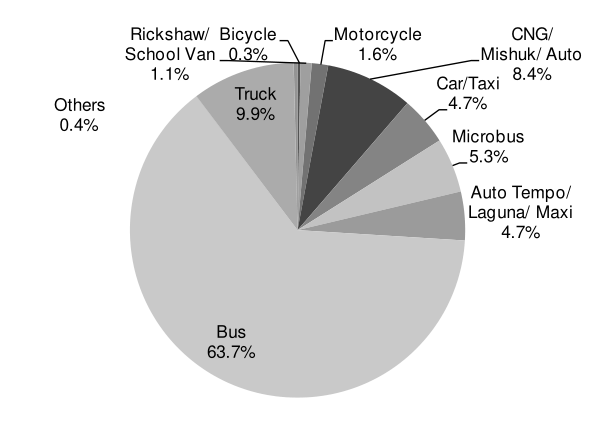
\includegraphics{./figures/rstp_modal_share_passenger.png}  
  \caption{Modal share of passenger} 
\end{center}
\end{wrapfigure}

The consequence is not very palatable here. As a result, many buses
enter into the same route, more popular routes, where many passengers
are available. There they heavily compete for passengers and results in
accidents and total chaos on the roads.

Overlapping bus routes from page 150 of \textcite{dtca_rstp_2015}

\hypertarget{consequence-of-competition}{%
\section{Consequence of competition}\label{consequence-of-competition}}

The competitive nature of the mass transportation in Metropolitan Dhaka
lowered the standard compared to other cities in the world . Following
is the direct quote from \textcite{dtca_utp_2015}:

``The transport systems in Metropolitan Dhaka are not only below
standard compared to many other capital cities, but they have reached
the crisis point that requires an immediate attention. A joint effort is
needed from all concerned to resolve the transport problem of the
city.'' This report identifies several consequences related to this poor
state of mass transportation.

This competition among bus companies results in aggressive driving among
the drivers. They compete with each other to collect passengers to
increase revenue.This results in increased number of accidents on the
streets. The incident mentioned above is exactly the consequence of this
sort of situation.

Not only that, this high level competion is not auguring well for the
whole of the bus industries. Bus business is not very profitable at all.
As found in \textcite{rahman_business_2017}, the current bus business
model, the bus owners are operating at 30\% loss against benchmark
costs. The interestesting fact here is that the competition does not
result in improvement in the quality of buses. Rather it results in
lower quality. This because due to current bottlenecks, mainly traffic
congestion, the buses can not make enough trips to render it as
profitable venture. Therefore, they cut costs by reducing qaulity of
service, paying lower wages to driver, reducing maintenance cost. It
becomes a race to the bottom.

Firstly, there is high frequency of deaths, injury and property damages.
It results into serious loss of productivity and imparts a great burden
on the economy and social cost in terms of family trauma and in social
relationship. Due to these damages, it has been estimated that each year
US\$700 is lost which is 3\% of the GDP. There are many reasons for this
loss but directly results from competition is poor driving capabilities,
defective vehicles. As argued above, competition resulted in lower price
which was achieved by lower quality. These road accident, casualties and
collisions are direct result of number and quality of vehicles on the
road.

\hypertarget{number-of-accidents}{%
\paragraph{Number of accidents}\label{number-of-accidents}}

2000 2001 2002 2003 2004 2005 2006 2007 2008 2009 2010 2011 2012 2013
852 519 876 828 668 496 603 565 642 525 458 400 372 341 Source: Accident

There is many evidences of such poor quality of service:

\begin{wrapfigure}{l}{.4\textwidth}  
 \begin{center}
    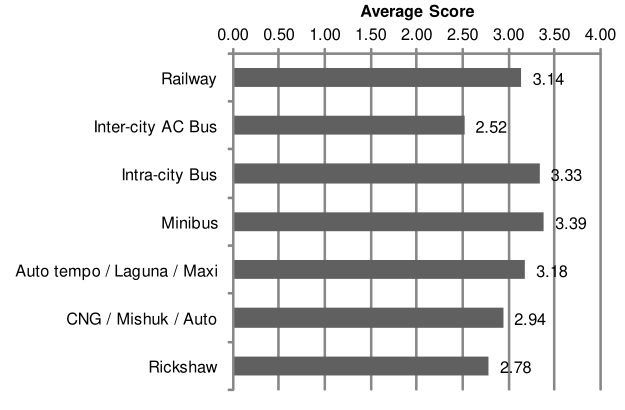
\includegraphics{./figures/rtsp_evaluations.png}  
  \caption{Passenger evaluation} 
\end{center}
\end{wrapfigure}

Then the pertinent questions that might arise in this case is that how
Buses attract passengers still with such low quality of service. This is
because mass transportationn is such service that the nature of demand
changes within hours. For example, during the peak demand or rush hour,
passengers will not mind quality that much, as long as quality is lower,
they will jump over and try to go to any place. Therefore, bus drivers
can get away with very low quality mass transit service. This is also
intrisically related to average income level of Bangladesh in general.
In this bus services, mainly low income people rides. The wealthy people
actually resort to Uber, Pathao or just their own car.

\begin{wrapfigure}{r}{.3\textwidth}  
 \begin{center}
    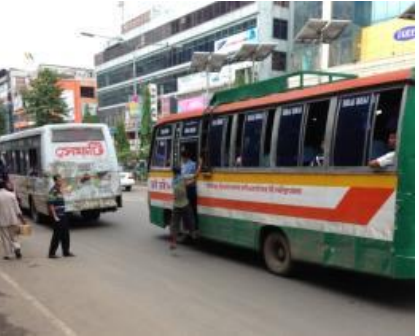
\includegraphics{./figures/rtsp_bus_condition1.png}  
  \caption{Bus condition} 
\end{center}
\end{wrapfigure}

Talking about personal car, this mode of vehicle has risen
astronomically due to reliable mass transport and unregulated
supervision of authority. \textbf{Provide some evidence here}. This is
also a severe consequence of lack of quality mass transit which was
caused by competitive nature of the bus service.

Talking about personal car, this mode of vehicle has risen
astronomically due to reliable mass transport and unregulated
supervision of authority. \textbf{Provide some evidence here}. This is
also a severe consequence of lack of quality mass transit which was
caused by competitive nature of the bus service.

\begin{wrapfigure}{l}{.3\textwidth}  
 \begin{center}
    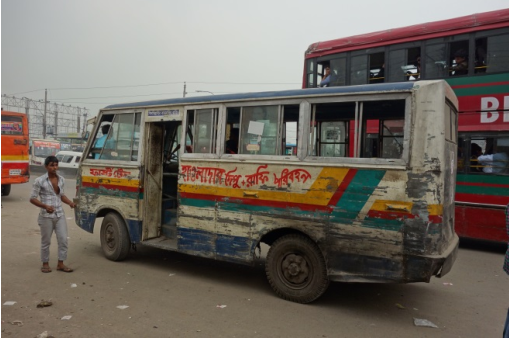
\includegraphics{./figures/rtsp_bus_condition2.png}  
  \caption{Bus condition} 
\end{center}
\end{wrapfigure}

Talking about personal car, this mode of vehicle has risen
astronomically due to reliable mass transport and unregulated
supervision of authority. \textbf{Provide some evidence here}. This is
also a severe consequence of lack of quality mass transit which was
caused by competitive nature of the bus service.

Talking about personal car, this mode of vehicle has risen
astronomically due to reliable mass transport and unregulated
supervision of authority. \textbf{Provide some evidence here}. This is
also a severe consequence of lack of quality mass transit which was
caused by competitive nature of the bus service.

Talking about personal car, this mode of vehicle has risen
astronomically due to reliable mass transport and unregulated
supervision of authority. \textbf{Provide some evidence here}. This is
also a severe consequence of lack of quality mass transit which was
caused by competitive nature of the bus service.

Talking about personal car, this mode of vehicle has risen
astronomically due to reliable mass transport and unregulated
supervision of authority. \textbf{Provide some evidence here}. This is
also a severe consequence of lack of quality mass transit which was
caused by competitive nature of the bus service.

Talking about personal car, this mode of vehicle has risen
astronomically due to reliable mass transport and unregulated
supervision of authority. \textbf{Provide some evidence here}. This is
also a severe consequence of lack of quality mass transit which was
caused by competitive nature of the bus service.

Talking about personal car, this mode of vehicle has risen
astronomically due to reliable mass transport and unregulated
supervision of authority. \textbf{Provide some evidence here}. This is
also a severe consequence of lack of quality mass transit which was
caused by competitive nature of the bus service.

\begin{wrapfigure}{r}{.4\textwidth}  
 \begin{center}
    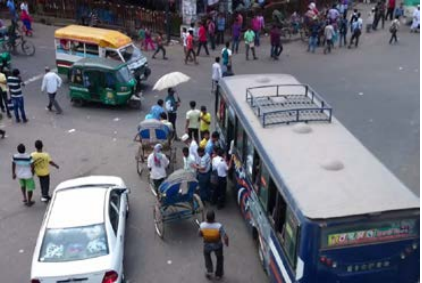
\includegraphics{./figures/rtsp_bus_condition3.png}  
  \caption{Bus condition} 
\end{center}
\end{wrapfigure}

Talking about personal car, this mode of vehicle has risen
astronomically due to reliable mass transport and unregulated
supervision of authority. \textbf{Provide some evidence here}. This is
also a severe consequence of lack of quality mass transit which was
caused by competitive nature of the bus service.

Talking about personal car, this mode of vehicle has risen
astronomically due to reliable mass transport and unregulated
supervision of authority. \textbf{Provide some evidence here}. This is
also a severe consequence of lack of quality mass transit which was
caused by competitive nature of the bus service.

\hypertarget{why-competition-does-not-work}{%
\section{Why competition does not
work}\label{why-competition-does-not-work}}

\textcite{ezrachi_curious_2015}, explains that commpetition and quality
are not positively correlated. Sometimes increase in competition can
actually reduce consumer welfare. They have identified two necessary but
not sufficient conditions for competition to work. Having these
conditions at their disposal, they described situations when an increase
in competition can acually may lead to quality degradation.

They identify two conditions: first it is prohibitively expensive or
difficult to convey consumers the inherent quality differences in the
product offering, and secondly, consumers' ability to accurately asess
quality differences is limited. In this regard, they mention that this
problem does not arise in the case of `search goods'. For these type of
goods, the consumers can check and evaluate the quality of the product.
But consumers does not have this advantage in the case of ``experience
goods'' for which the consumers have to learn the qulity by experiencing
the use of that particualr product. There is another type of good is
also mentioned which is called ``credence good'', I am not sure what
does that mean actually.

The problem is that the above two conditions may not be applicable in
the particular case of buses in Dhaka city. This is because buses are
`experience goods' and passengers experience that every day. But as
mentioned above, even though the passengers experience low quality
products, they just can not afford to lose the transportation during the
peak hour due to huge demand.

Therefore, there are certain goods and services which create highly
disparate demand in daily different time intervals. Bus companies does
not invest highly in those buses because they know that they can away
with low quality products. They make their major businesses during this
peak hour. The thing is there due to traffic congestion they cannot make
enough profit. One the other hand, they can not charge high due to
competition. Only way they can survive is that by cutting costs which
results in lower quality.

\hypertarget{concluding-remarks}{%
\section{Concluding remarks}\label{concluding-remarks}}

\printbibliography[title=References]

\end{document}
